\subsection{Sistemas implicados} 

Aunque previamente hemos comentado la idea de que no todas las instalaciones valen para todos los tipos de antenas, es en este punto donde debemos destacar la importancia de esto.\\ 

Y es que, los requisitos para poder tomar medidas varían notablemente en función del tipo de antena que deseamos medir. Ya que los requisitos necesarios para caracterizar una antena pasiva de un solo puerto serán menos exigentes que los necesarios para medir una esfera de antenas de múltiples puertos usada para comunicaciones inalámbricas de alta velocidad. 
\\

Por lo que, frente a la posibilidad de tener que construir una arquitectura totalmente nueva para cada tipo de antena. Se decidió plantear un modelo lo más generalista posible. El cual encontramos definido en el estándar 149-2021 y toma la siguiente forma
\newpage

\begin{figure}[h]
    \centering
    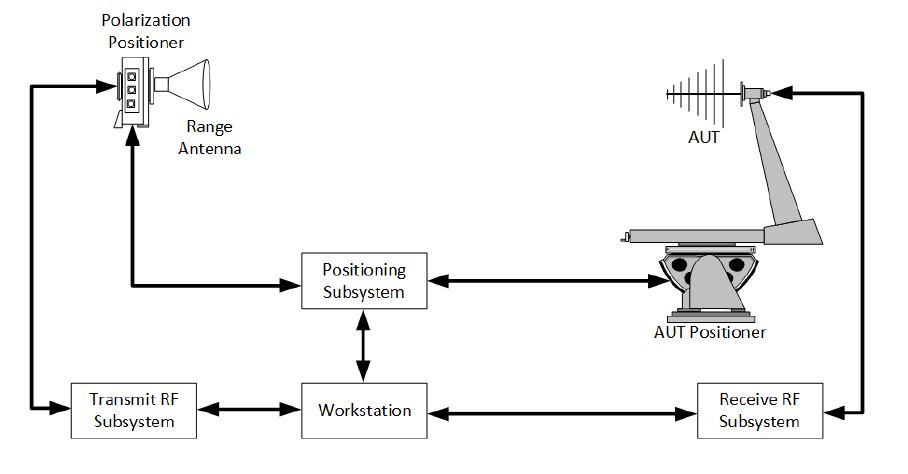
\includegraphics[scale=0.65]{Figura3-Modelo de una estacion completa de medidas}
    \caption{Modelo general de una estación de medidas.}
    \label{Modelo-general-de-una-estación-de-medidas}
\end{figure}

Este es el modelo de que disponemos y que vamos a explicar en esta sección. No sin antes hacer una aclaración con respecto a los contenidos que vamos a ver. Y es que cada uno de estos sistemas son, por si solos, objetos de estudio en sí mismos. Por lo que entrar en profundidad en su funcionamiento excede los contenidos a tratar en este documento.
\\

El objetivo de lo visto en esta sección es tener el contexto suficiente de cómo funciona y se comporta cada sistema. De manera que entendamos de dónde vienen ciertas limitaciones o porqué debemos usar ciertos sistemas de coordenadas. Vitando en la medida de lo posible detallar conceptos ajenos a nuestro campo de estudio. 

\subsubsection{Sonda} 

Si nos fijamos en la figura \ref{Modelo-general-de-una-estación-de-medidas}, nos encontramos con un elemento sobre el que no hemos hablado hasta ahora. La antena transmisora.\\
Hasta ahora únicamente hemos hablado de que para medir una antena requeríamos poder transmitir una onda plana uniforme; y del hecho de que en la realidad no es posible generar una onda plana perfecta. Pero no comentamos nada relacionado con como íbamos a transmitir dicha onda. Cosa que vamos a abordar en esta sección. 
\\

El uso de esta antena, denominada sonda de ahora en adelante, es necesario para poder transmitir nuestra onda plana a la AUT y así poder obtener medidas. Lo que supone que, en aras de poder conocer el comportamiento de la antena bajo test, debemos conocer a la perfección el comportamiento de nuestra sonda.
\\

Otro concepto a destacar del uso de la sonda, es la idea de que nuestro sistema de medidas pivota sobre dos antenas. Por lo que se dan diferentes configuraciones posibles en función de donde se sitúan la sonda y la AUT. Existiendo configuraciones donde están en posiciones fijas, como la ilustrada en la figura \ref{Modelo-general-de-una-estación-de-medidas}. O en las cuales se puedan intercambiar de posición. Existiendo incluso algunas instalaciones usan sistemas más pequeños cuya arquitectura combina la sonda y la AUT en una misma unidad. 
\\

No obstante, independientemente de la configuración ante la que estemos, el funcionamiento de cada sistema es idéntico. Por lo que todo lo visto a continuación es válido independientemente de dónde estén situadas las antenas. 

\subsubsection{Frecuencia de trabajo}

A excepción de algunas instalaciones especializadas en ciertos tipos de medida. Es habitual que las instalaciones de medida se diseñen para usar un rango de frecuencia lo más amplio posible que cumpla los límites aceptables de funcionamiento. Los cuales ya hemos visto cuales son y cómo calcularlos.
\\

Sin embargo, operar sobre un rango amplio de frecuencia trae consigo un problema principal. Ya que usualmente este rango de frecuencia excede el ancho de banda de trabajo de nuestra sonda. 
\\

Para solventar esto, es habitual disponer de una familia de antenas que en conjunto si permitan cubrir dicho rango de frecuencias. Lo que supone disponer de un grupo de antenas que debe tener una ganancia, ancho de haz y polarización coherentes con las medidas que queremos realizar nuestro rango.\\
Ya que no todas las antenas disponen de los mismos requisitos de línea de visión, reflexión o rangos compactos.
\\

Otro aspecto a tener en cuenta es que deseamos caracterizar la AUT en ambas polarizaciones, horizontal y vertical. Por lo que necesitamos una forma de controlar la polarización que usamos en nuestra sonda. Para esto, se suele optar por usar sondas polarizadas de forma ortogonal. Aunque también es habitual montar una sonda de polarización lineal sobre un posicionador de polarización. Lo cual permite orientar el ángulo de inclinación de la polarización.

\newpage

\subsection{Subsistema de Transmisión}

La función principal del subsistema de transmisión es generar pequeñas señales de forma controlada para estimular la antena bajo estudio. Motivo por el cual necesitamos tener muy acotados los niveles de frecuencia y potencia. 
\\

Para poder cumplir con este requisito, la selección de componentes del subsistema de transmisión depende mayoritariamente de criterios como el rango de frecuencias, el nivel de potencia a transmitir o el aislamiento. Para lo cual se suele hacer uso de una fuente que genere la señal a transmitir, un acoplador de referencia, un multiplicador de frecuencia y amplificadores. 

\subsection{Subsistema de recepción}

El propósito de este subsistema es medir la respuesta de la AUT para cada ángulo de recepción posible. Por lo que el criterio para elegir los componentes de este sistema se centra en garantizar la mayor fidelidad posible en la medición. 
\\

Centrándonos un poco en los instrumentos de medida, existen dos grupos principales: 

\begin{itemize}
    \item \textbf{Instrumentos escalares:} Son aquellos instrumentos capaces de realizar medidas en amplitud. Incluyéndose en este grupo, por ejemplo, los medidores de potencia y los analizadores de espectro. 
    \item \textbf{Instrumentos vectoriales:} Paralelo a los escalares, son aquellos instrumentos capaces de realizar mediciones de amplitud. Incluyéndose en este grupo, por ejemplo, los analizadores vectoriales de redes o los receptores de medida. 
\end{itemize}
No obstante, en la mayoría de las instalaciones modernas se mide tanto en amplitud como en fase mediante el uso de analizadores de redes vectoriales. Motivo por el que vamos a centrándonos en este tipo de instrumentación. 

\newpage

\begin{figure}[h]
    \centering
    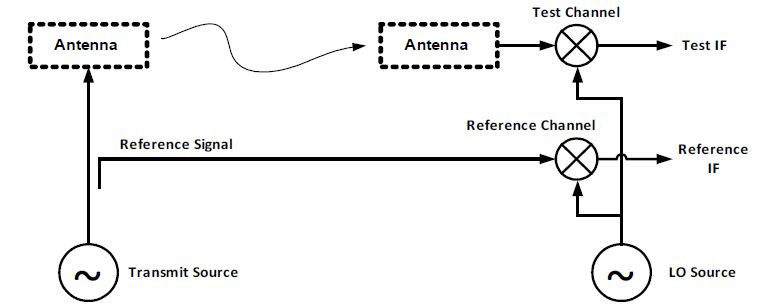
\includegraphics[scale=0.65]{Figura4-Elementos subsistema de recepcion}
    \caption{Elementos clave de un sistema de medición vectorial típico.}
    \label{Elementos-subsistema-de-recepcion}
\end{figure} 

Lo primero que podemos destacar del diagrama. Es el uso de dos canales para la medida de la fase en la AUT.\\
Uno de estos canales, el denominado canal de referencia del receptor, porta la señal de referencia generada por el subsistema de transmisión. Mientras que el otro canal, denominado canal de medición, es el que se conecta a la antena receptora y empleamos como canal de pruebas. 
\\

La respuesta en fase de la AUT se obtiene entonces midiendo la fase existente entre estos dos canales. Motivo por el cual es imperativo trabajar con la misma frecuencia en ambos canales. Para esto, se hace uso de un oscilador local común a los dos canales. Permitiendo convertir los canales a una frecuencia intermedia fija que permite digitalizar y procesar las señales. 
\\

En cuanto a la medida de amplitud. Se tiende a hacer uso de la relación de amplitud entre los dos canales. Ya que el uso de esta relación ayuda a minimizar los efectos debidos al desplazamiento de amplitud del subsistema de transmisión. 
\newpage

\subsection{Subsistema de posicionamiento} 

En el punto anterior hemos mencionado que el subsistema de recepción debe ser capaz de recibir medidas para todos los ángulos posibles. Lo cual es posible gracias a este subsistema, que es el encargado de controlar la orientación tanto de la sonda como de la AUT. 
\\

Esto supone que debe ser capaz de gestionar la carga de las antenas manteniendo a la vez la precisión de la toma de medidas. Además de introducir por primera vez la necesidad de emplear un sistema de coordenadas concreto asociado a dichas medidas. 
\\

Esto se detalla más en profundidad en las explicaciones de las transformaciones que permiten obtener el campo lejano. Pero típicamente se usa el sistema de coordenadas esféricas. Que es el que vamos a considerar aquí. 
\\

Independientemente de si la línea de visión es fijas o móvil, necesitamos disponer de dos ejes ortogonales que combinados permitan efectuar cortes en $\theta$ y $\phi$. Estos ejes se designan como el eje de rotación $\theta$ y el eje de rotación $\phi$. Los cuales están representados en la siguiente figura. 

\begin{figure}[h]
    \centering
    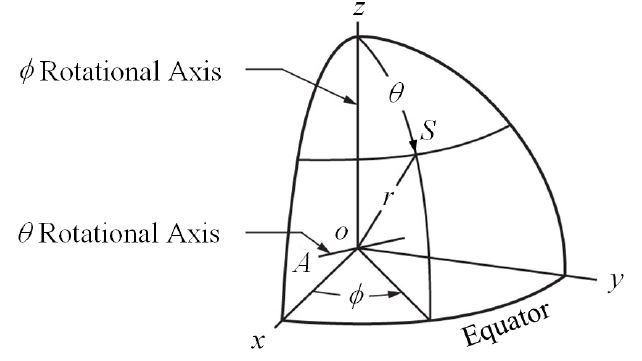
\includegraphics[scale=0.5]{Figura6-Ejes ortogonales para medir antenas}
    \caption{Ejes de rotación en un sistema esférico.}
    \label{Ejes-ortogonales-para-medir-antenas}
\end{figure} 

En nuestro caso particular, la sonda está fija y haremos pivotar la AUT de forma que podamos tomar medidas en un rango significativo de ángulos.

\newpage